\section{Methods}

\subsection{Overview}

Our hypothesis is that performing test time adaptation on cell segmentation will improve cell tracking performance since the associations are based on simple metrics such as IoU and Euclidean distance of the centroids. We propose to pretrain a denoising framework that takes three inputs: The raw image, noisy segmentation from a pretrained segmentation model, and Gaussian splats retrieved from the raw image, and produce a clean segmentation mask as pseudo labels.
Once the pseudo labels are retrieved, we perform knowledge distillation with stochastic restoration of parameters to perform the test-time adaptation. Please refer to \Cref{fig:overall_framework}.


\begin{figure}[t]
    \centering
    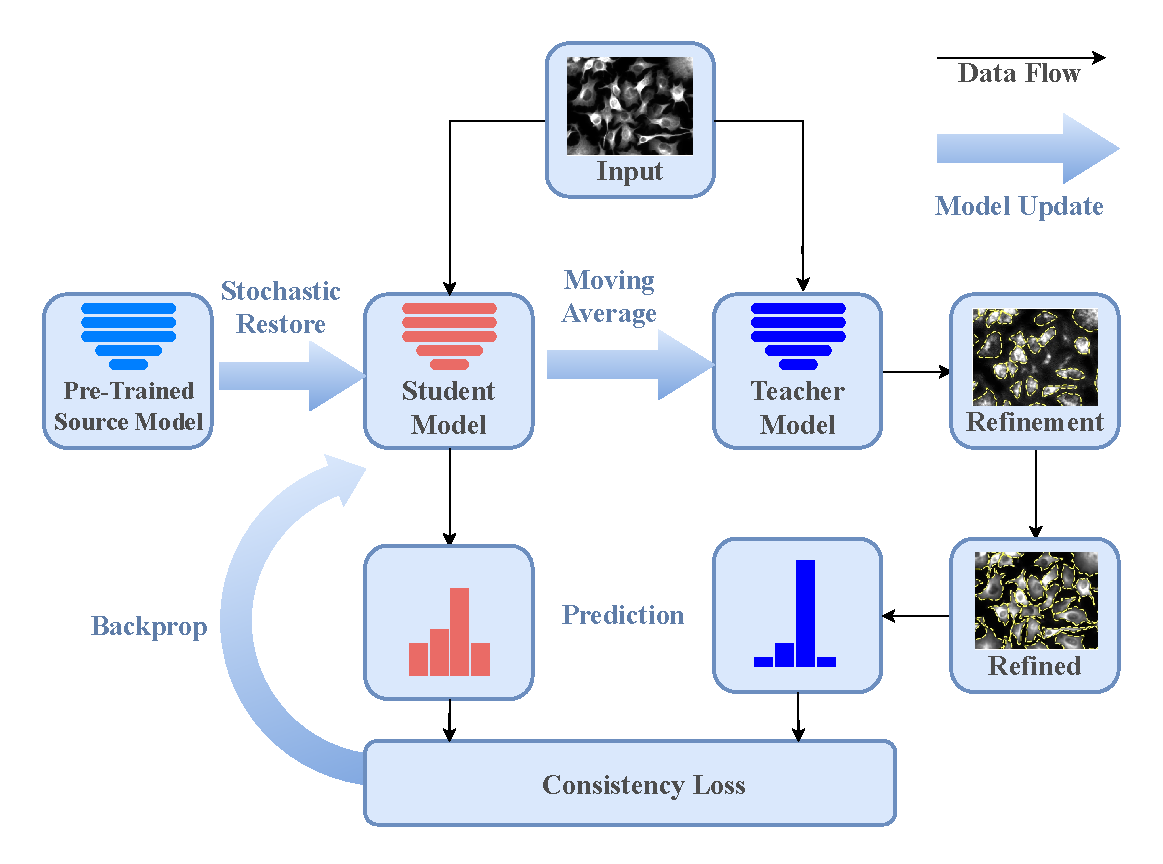
\includegraphics[width=9cm]{figs/project_proposal.pdf}
    \caption{Overall Framework.}
    \label{fig:overall_framework}
\end{figure}

\subsection{Cell Segmentation}

To test our hypothesis, we use one of the state-of-the-art cell instance segmentation algorithms as our segmentation framework Cellpose~\cite{stringer2021cellpose}. It is pretrained on diverse datasets and has good generalization capability. However, it is not pretrained on all imaging modalities or cell types, rendering it less useful in out-of-distribution datasets. We propose to utilize their pretrained model and perform test-time adaptation. 

\subsection{Training Gaussian Splats Algorithm}

Radiance fields are a new form of 3d representation which relies on novel differentiable ray-marching, in this talk we will discuss two types Neural Radiance Fields (NeRF) and Gaussian Splatting (GS).   In brief, a radiance field is a learnable representation of a scene, in the case of the NeRFS a large MLP is used as the mechanism and in GS a variable list of ellipsoids.  A raycast is a form of graphics rendering in which the emission of photons onto a pixel is calculated by tracking the reflection of light.  For instance, to find the color of the middle pixel of an image, a ray can be calculated in the opposite direction of how light is received by the camera.  Usually in the case of raycast, for simplicity, once the ray hits an object in the 3d scene it stops and the color of the hit object is blended into that pixel.  \\

Instead of the ray cast ending after an arbitrary number of reflections, the rays’ direction is not affected by reflection.  Each perceptron in NeRF or Ellipsoid in GS is associated with an emission of light which adds its contribution to the ray by integrating the contribution of each perceptron or ellipsoid to the ray small changes to the light emitted are captured by the alpha-blending equation.  \\

Each of these are trained by taking training samples and finding the divergence between the rendering at the current training step compared to the known ground truth image.  In order, to have this information though you need to also know the pose of the camera relative to the scene during training which can be a major impediment to applying a radiance field method. In this case we have the benefit of a closed system where we can define the position of the viewer based on the geometry of the original imaging system which is published information.  \\

\subsection{Refinement}




\begin{figure}[t]
    \centering
    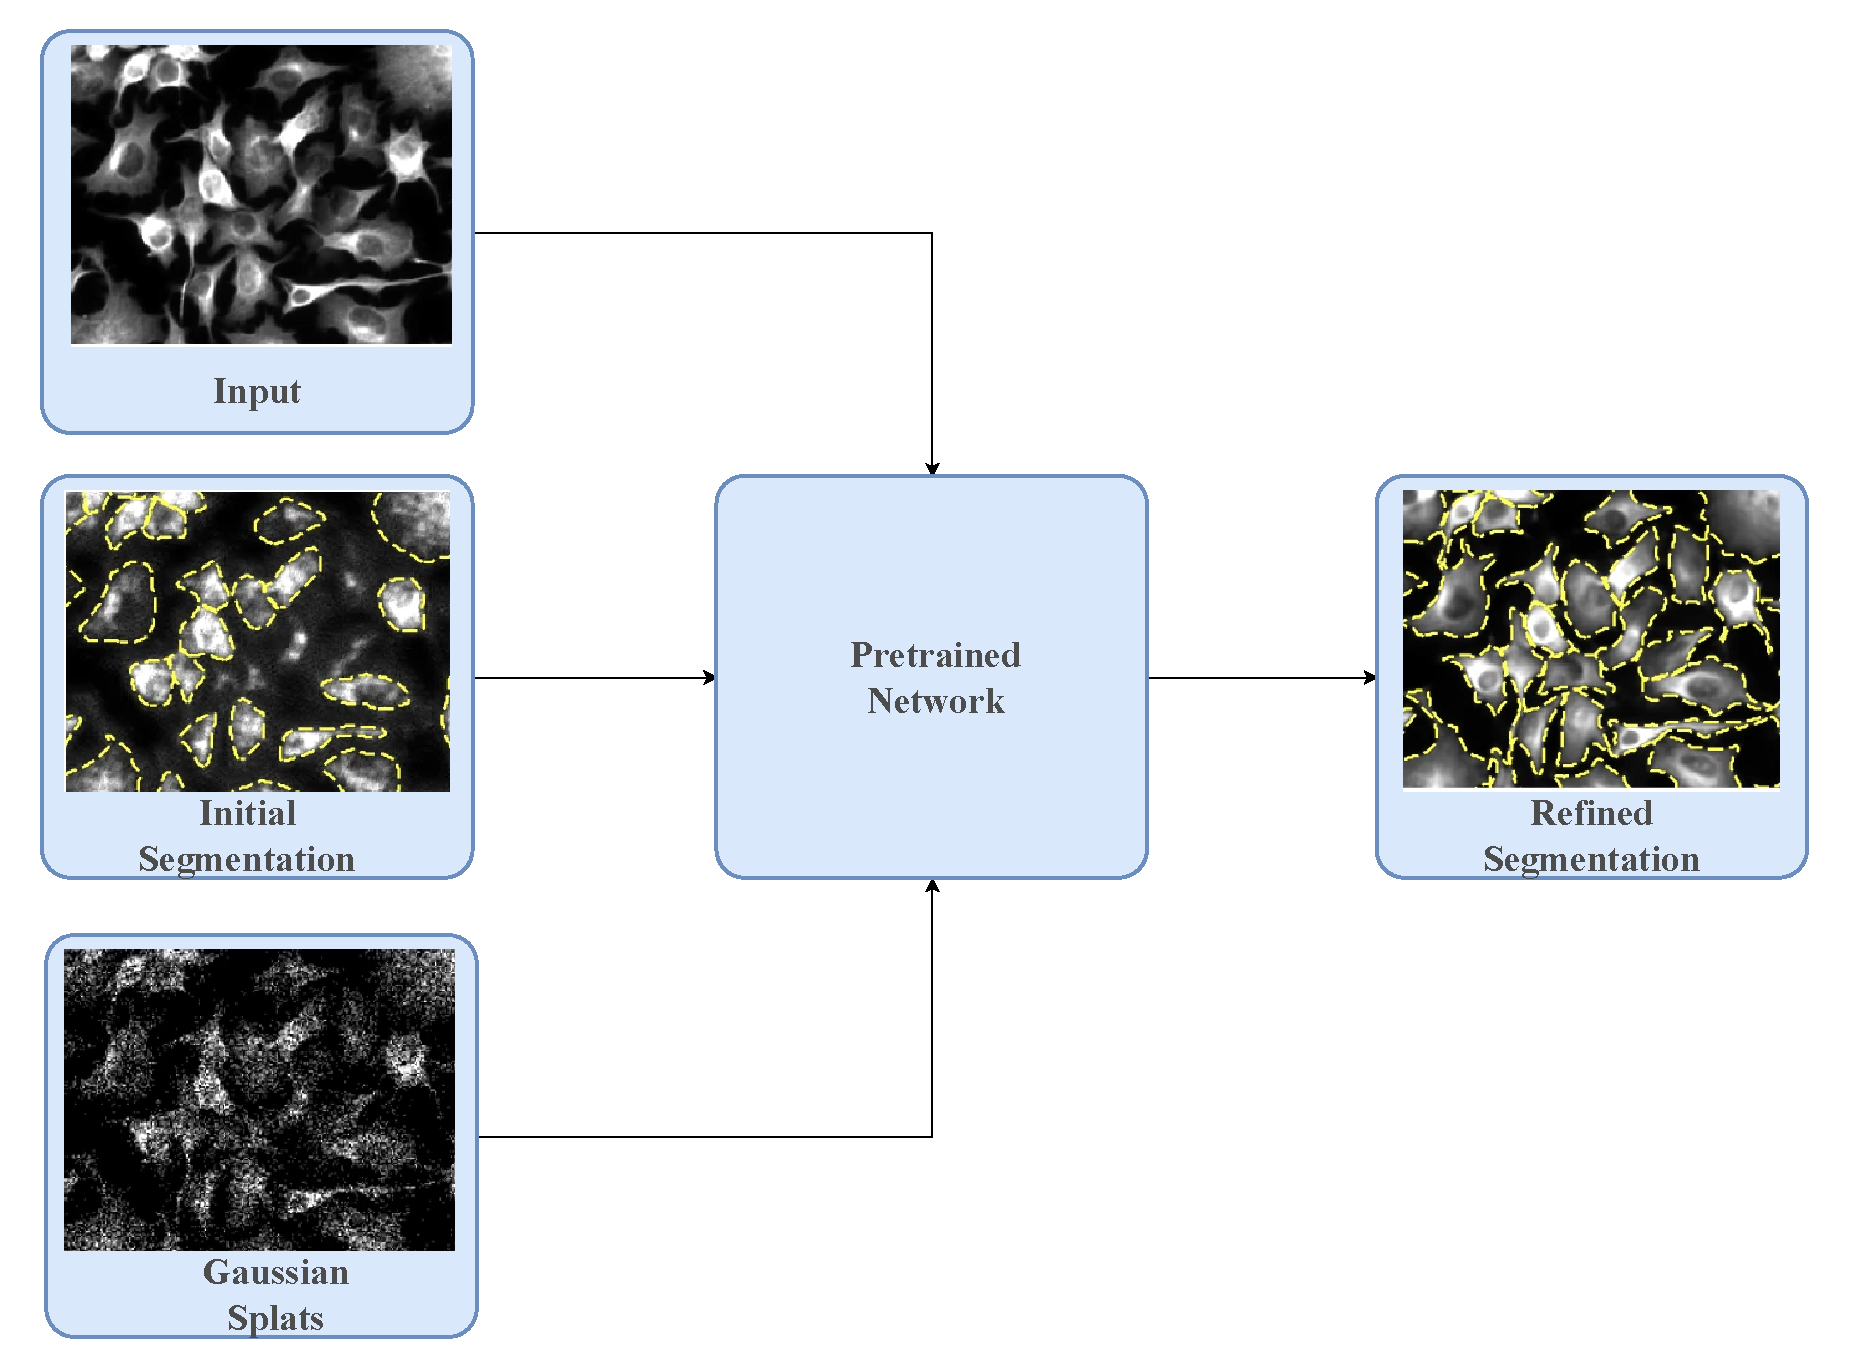
\includegraphics[width=9cm]{figs/refinement.pdf}
    \caption{Refinement Strategy.}
    \label{fig:refinement}
\end{figure}

\subsection{Test-Time Adaptation}

\subsection{Cell Tracking}